
\documentclass{IOS-Book-Article}

\usepackage{mathptmx}
\usepackage{soul}\setuldepth{article}
\usepackage{booktabs}
%\usepackage{times}
%\normalfont
%\usepackage[T1]{fontenc}
%\usepackage[mtplusscr,mtbold]{mathtime}
%
\usepackage{multirow}
\usepackage[table]{xcolor}
\usepackage{colortbl}
\usepackage{multirow}
\usepackage{numprint}
\usepackage{graphicx}
\usepackage{hyperref}
%\renewcommand\UrlFont{\color{blue}\rmfamily}
\setlength{\parskip}{0pt}
\raggedbottom
\usepackage{multirow}
\usepackage{amsmath}
\usepackage{csquotes}
\usepackage{paralist}
\usepackage{booktabs}
\usepackage{mathptmx}
\def\hb{\hbox to 10.7 cm{}}
\usepackage{pgfplots}
\pgfplotsset{compat=1.8}
\usepackage{subfigure}
\pgfplotsset{width=7cm,compat=1.8}
\usepackage{pgfplotstable}
%\renewcommand*{\familydefault}{\sfdefault}
\usepackage{tikz}
\def\hb{\hbox to 10.7 cm{}}
\begin{document}

\pagestyle{headings}
\def\thepage{}

\begin{frontmatter}              % The preamble begins here

%\pretitle{Pretitle}
\title{On the efficiency of Machine Learning Models in predicting Malaria using Sympt\^om Data}

\markboth{}{January 2020\hb}
%\subtitle{Subtitle}

\author{\fnms{Ousseynou} \snm{Mbaye}},
\author{\fnms{Mouhamadou Lamine} \snm{BA}
\thanks{Corresponding Author: Mouhamadou Lamine BA, LIMA, Universit\'e Alioune Diop,
BP.3400 Bambey, Senegal; E-mail: mouhamadoulamine.ba@uadb.edu.sn.}}
and
\author{\fnms{Alassane} \snm{SY}}

\runningauthor{O.Mbaye et al.}
\address{LIMA, Universit\'e Alioune Diop, Bambey, Senegal}
%\address[B]{Short Affiliation of Second Author and Third Author}

\begin{abstract}
Still today, Malaria remains one of the most feared diseases in Sub-Saharan Africa and especially in Senegal. This is mainly due to inappropriate medical care support coupled with an often late and error-prone diagnosis from the medical staff. In addition, largely used diagnostic standards such as the Rapid Diagnosis Test is not fully reliable. With the development and increasing adoption of automated tools in the health field, machine learning applications might help medical actors in their decision-making process. In this paper, we propose an experimental study of six machine learning algorithms for the prediction of Malaria in Senegal. These algorithms aim at predicting whether or not a given patient suffers from Malaria based on his signs and symptoms. The performance of the algorithms have been extensively tested and evaluated over real data sets about patients in Senegal that suffer or not from Malaria. The algorithms are evaluated using four criteria: accuracy, Recall, F-measure, Precision and Specificity. The research has shown that there is not necessarily a single best classification tool, but instead the best performing algorithm will depend on the dataset to be analysed.
\end{abstract}

\begin{keyword}
electronic camera-ready manuscript\sep IOS Press\sep
\LaTeX\sep book\sep layout
\end{keyword}
\end{frontmatter}
\markboth{January 2020\hb}{January 2020\hb}
%\thispagestyle{empty}
%\pagestyle{empty}

\section{Introduction}\label{Introduction}
Malaria is a transmissible disease through the bites of infected female Anopheles mosquitoes. It comes with symptoms such as fever, headache, and chills in its early stage and can evolve to more severe health problems (severe anaemia, respiratory distress, etc.) often leading death. In 2019, the number of Malaria cases worldwide has been estimated to 229 millions. The number of deaths caused by Malaria has been approximatively estimated to 409 000 in 2019; the African area represents around 94\% of the reported malaria cases and deaths in 2019, thanks to the annual world Malaria report \cite{19WMR}. 

Over the past years, many efforts have been made by governmental and non governmental organizations (e.g. WHO) to eradicate Malaria in the world.  In the research field, many studies, aiming at understanding the disease from the Plasmodium mosquito point of view or proposing automated detection tools, have been conducted \cite{Ga19,Le74,ermert2011development,Hu17}. The Rapid Diagnostic Test (RDT) \cite{Hu17} is one of the most successful and prominent introduced tool to automatically predict whether or not a given patient suffers from Malaria. It relies on the detection of the presence of specific Plasmodium proteins, PfHRP2, pLDH
and aldolase in human blood. The RDT is largely used and adopted as a standard many Sub-saharan African countries such as Senegal. However, as proved in \cite{Hu17}, RDT is not fully reliable:  Section \ref{Methods} shows that the precision of RDT is about 90\% for datasets used in this study. Despite those advanced tools, Malaria is still a real public health in sub-Saharan African countries such as Senegal because of the lack of appropriate care support or late and error-prone detection of the disease.
Artificial intelligence is now recognized as a domain that may help medical actors in their decision-making process. \cite{mitchell1997machine, Ug1}  
 This paper proposes an  extensive comparative study of the most popular machine learning models for the task of Malaria prediction. The evaluated and compared ML algorithms are Naive Bayes (NB), Logistic Regression(LR),  Decision Tree(DT), Support Vector Machine(SVM) ,
 Random Forest(RF), and Artificial Neural Network(ANN). We conducted experiments on five datasets about patients living in Senegal. The raw
 datasets have been collected in different settings and contain clinical data such as sign, symptom and the diagnostic of the doctor.  The outcome of the RDT is also provided. Our main result is that Random Forest, Logistic Regression, Support Vector Machine with Gaussian kernel and Artificial Neural Network outperforms RDT and present very high precision in the Senegalese patient datasets.
The rest of the paper is organized as follows. We start by presenting the methods used in this work in section \ref{Methods}. In section \ref{results_discussion} details the results of the intensive experimentations conducted over various datasets. Finally, we conclude this paper in section \ref{conclusion}.


% Prediction Model
\newpage
\section{Methods}\label{Methods}
\subsection{Machine Learning algorithms in healthcare}
There are already some attempts to apply ML techniques for the prediction or a better understanding of various diseases, e.g. logistic regression has been tested in \cite{mbaye2019towards} for the prediction of Malaria and provides promising results.
\subsection{Datasets}
In order to carry out  our experiments in a real setting we have collected two real world datasets about patients living in Senegal. We describe each of them in the sequel.\\
\textbf{Data collection.} Our first dataset, that we  to refer to it as DT1, contains medical records about patients living in distinct places in Senegal. It has been collected in 2016 during the \textbf{Grand Magal of Touba}  which is one of the most popular religious event in Senegal. Such an event gathers every year several millions of persons that come from various areas around the country \cite{Ch17}.  During the event several fixed and mobile health points are set up to enable the examination and treatment of ill persons. The second dataset, denoted by DT2, has been collected by drawing our attention on medical records about patients living in the same area. We focused on the district of Diourbel,Thies and Fatick \footnote{https://en.wikipedia.org/wiki/Diourbel\_Region} where the prevalence of Malaria is very high and collected patient records from its different health structures. \\
\textbf{Data features.} Table \ref{raw_data} contains the main characteristic of each dataset. Some of these variables (also called features or attributes) include personal data about the patient, but also signs and symptoms(e.g. lack of appetite, tiredness, fever, cephalalgia, nausea,
arthralgia, digestive disorders, dizziness, chill, myalgia, diarrhea, and abdominal pain) of the patient reported by the doctor who treated this later. The other attributes describe clinical data such as information about the doctor's final diagnosis (the patient's disease), the outcome of the Rapid Diagnosis Test and the patient's status (i.e. admission, death or observation). For privacy reasons and certain restrictions in the use of the data, we have ignored patient personal data  during this study.
In addition, we can observe that  both datasets are unbalanced because the proportion of observations per class is largely unequal. As an example for dataset DT1 we have 614 observations in the first class and 5108 observation in the second class. Finally, we remarked that the precision of the Rapid Diagnosis Test is around 90\% for both datasets, meaning that the systematically performed RDT in Senegal is not fully reliable.
\begin{table*}[h]
\centering
  \begin{tabular}{cccccccc}
    \toprule
    \multirow{2}{*}{\textbf{Dataset}} &
      \textbf{Variables}&\textbf{Observations}&
      \multicolumn{2}{c}{\textbf{Variables types}}& \multicolumn{2}{c}{\textbf{Classes}} & \textbf{Precision of RDT}\\
    & & & Numeric & Boolean & Malaria & not Malaria \\
    \midrule
    DT1 &16 & 21083  & 2 &  14& 614&20469 & 90.23\% \\
    DT2 & 16 & 5809 & 2 & 14 & 5108&701 & 90.49\% \\
    \bottomrule
  \end{tabular}
  \caption{Raw Data characteristics}\label{raw_data}
\end{table*}

From DT1 and DT2 we built three news datasets DT3, DT4 and DT5 data sets as below.\\
\textbf{DT3:}  It is obtained by concatenating the DT1 and DT2 datasets. Thus it concerns 37,175 patients of which 9,837 are diagnosed positive for malaria.\\
\textbf{DT4:} It is obtained by considering the 16,092 patients in the DT2 data set (including 9,223 patients with malaria). Since this DT2 is unbalanced, we randomly selected 2354 patients who tested negative for malaria from the DT1 data set at the end of the rebalance. Thus it concerns 18,446 patients, 9,223 of whom are suffering from malaria.\\
\textbf{DT5:} is obtained by the over sampling of DT1 by the SMOTE method of python. This method consists first of dividing DT1 into two parts, one for training (train set) and the other for testing (test set). The train set being unbalanced, then we apply the SMOTE method to remedy it. Thus we obtain a new train set comprising 30,369 patients, half of whom tested positive for malaria.
\subsection{Machine Learning algorithms studies}
In the following we discuss about some of these methods.  Those algorithms are chosen among the most used ones in the health field according to studies\cite{de2018binary,tomar2013survey}.\\
\textbf{Decision tree (DT)}\cite{Ro05} is a supervised classifier which is obtained by recursively partitioning the labelled set of observations. It is one of the most adopted classifiers, thanks to its simplicity and its straightforward interpretation. For CART algorithms, hyperparameters are the impurity criteria (entropy and gini), the maximum depth, the minimum samples to split and the minimum samples at a leaf

% Random forest
Random Forest (RF) \cite{Be01}: RF is an ensemble approach built upon many decision tree classifiers. It is a supervised classifier which requires the same hyper parameters as DT, plus the number of trees to create and the random number of features to look at when splitting the labelled data during the training step \cite{Be01}.\\
% Naive Bayes
Naive Bayes classifier (NB): NB\cite{Ka17} is a\emph{supervised} machine learning algorithm, i.e. requires to be trained, used for classifying observations to given distinct classes based on \emph{input explanatory variables} (a.k.a feature or attribute).
It is a classification technique based on the well-known \emph{Bayes’ theorem}\footnote{https://en.wikipedia.org/wiki/Bayes\%27\_theorem} with strong and naive assumptions. It simplifies learning by assuming that features are independent of given class.\\
% Logistic Regression 
Logistic regression (LR: LR \cite{Ph88} is a statistical model used in the machine learning domain as a supervised classifier for binary classification \cite{uddin2019comparing}. 
It is based, in its basic form, on a logistic function to describe a binary dependent variable\cite{wang2014support,de2018binary} by considering as input 
qualitative or/and ordinal explanatory variables  in order to measure the probability of a given class label. \\
%Support Vector Machine
Support Vector Machine (SVM): SVM \cite{Ev01} is a supervised classification approach whose intuition is to represent input data in a space and to determine the optimal hyper-plane that divides that space in two regions depending on the targeted value.\\
% artificial neural networks
 Artificial Neural Network (ANN): ANN \cite{Me19} is a computational approach also referred to as a Connectionist System used in Machine Learning. ANNs are loosely modeled after the biological neural network in an attempt to replicate the way in which we learn as humans. Think of it as a computing system, structured as a series of layers, each layer consisting of one or several neurons. The types of the layers comprise \emph{input}, \emph{output} and \emph{hidden} layers \cite{anderson1972simple,raschka2015python}.
\subsection{Experimentation Setting}
In this section data is available for applying classification algorithm. After model creation from training data, classification operation is performed on test data. 
All the performed tests have been done in the same machine and the same operating system. To test the performance of our six chosen ML algorithms, we relied on their Python implementations available through the scikit-learn library. Scikit-learn is an open source simple and efficient tool for predictive data analysis that implements most of the existing ML algorithms.
For the details about the description of each parameter of ML we refer to the official documentation of the implementation of these algorithms in scikit-learn7. Concerning the segmentation of both datasets for the training of our ML algorithms and their testing we have considered the stratified-5-fold cross-validation in classification model construction and efficiency evaluation. This method is very useful to handle data with an unbalanced class distribution, increases the validation of classification and prevents from random and invalid results.
\subsection{Measurement} 
To evaluate the performance of every considered algorithm we have considered common measures of the accuracy of a prediction system that are \emph{Precision}, \emph{Recall}, \emph{F1-score}, \emph{True Positive Rate}, and
 \emph{False Positive Rate} on both datasets augmented with semi-synthetic datasets which are obtained after imputation in order to deal with missing values.
% Related work
\section{Results of the experiments}
Table \ref{raw_data1} presents the results of the experiments with the different algorithms on our data on Malaria. More specifically, Table 2 contains the precision, the recall, the specificity, the AUC mesure, the score and F-measure of each algorithm tested while Figure 1 shows their respective ROC curve.  
\begin{table}[h]
\begin{tabular}{|l|c|c|c|c|c|c|c|}
\hline
\cline{2-8}
 \textbf{ML ALgorithms} &  \textbf{Datasets} & \textbf{Precision} & \textbf{Recall} & \textbf{F1-score}&\textbf{AUC} &\textbf{Score}&\textbf{Specificity}\tabularnewline
\hline
\cline{2-8}
 &  DT1 &0.97  & 1   & 0.98 & 0.78 & 97.04 & 0.05 \\
\cline{2-8}
& DT2 & 0.59 &0.48 &0.48  &0.64  &63.01  &0.80\\
\cline{2-8}
& DT3 &0.89  &0.85 &0.87  &0.86  &80.86  &0.69\\
\cline{2-8}
& DT4 &0.68  &0.57 &0.62  &0.70  &65.60  &0.74\\
\cline{2-8}
\multirow{-4}{*}{ \textbf{Decision Tree}}&   DT5 &0.99  &0.84 &0.91  &0.76  &83.41  &0.58\\
\hline
\cline{2-8}
&DT1 &0.97 &1   &0.99 &0.81 &97.13& 0.07\\
\cline{2-8}
 & DT2 &0.63  & 0.34  &0.44&0.64&63.33& 0.85\\
 \cline{2-8}
 & DT3 &0.89 &0.85 &0.87&087&80.86&0.70\\
 \cline{2-8}
 & DT4 &0.68 &0.56&0.62&0.70&65.82&0.74\\
\cline{2-8}
\multirow{-4}{*}{ \textbf{Random Forest}}&   DT5 &0.99 &0.84&0.91&0.76&78.35&0.60\\
\hline
\cline{2-8}
&DT1 &0.97 &1   &0.99 &0.79 &97.19&0.05 \\
\cline{2-8}
 &DT2 & 0.58 &0.36   &0.44&0.63&61.96&0.81\\
 \cline{2-8}
  &DT3 &0.85 &0.88 &0.86&0.86&79.59&0.55\\
  \cline{2-8}
  &DT4 &0.98 &0.56&0.92&0.70&65.82&0.72\\
  \cline{2-8}
\multirow{-4}{*}{ \textbf{Logistic Regression}}&   DT5 & 0.90&0.78&0.88&0.84&81.86&0.75\\
\hline
\cline{2-8}
& DT1 &0.97 &1   &0.99 &0.81 &97.13 &0.00\\
 \cline{2-8}
  &DT2 & 0.60 &0.34   &0.43&0.63&62.86&0.83 \\
  \cline{2-8}
  &DT3 &0.86 &0.87 &0.86&0.85&79.94&0.60\\
  \cline{2-8}
  &DT4 &0.68 &0.59&0.63&0.70&65.63&0.73\\
  \cline{2-8}
\multirow{-4}{*}{ \textbf{Naive Bays}}&0.99 &0.82&0.90&0.84&85.61&0.71&0.71\\
\hline
\cline{2-8}
&DT1 &0.97 &1   &0.99 &0.84 &97.13&0.00 \\
\cline{2-8}
  &DT2 &0.58  &0.05   & 0.09&0.62&62.86&0.97\\
  \cline{2-8}
  &DT3 &0.57 & 0.86&0.86&0.85&79.94&0.64\\
  \cline{2-8}
 & DT4 & 0.68&0.58&0.62&0.70&65.63&0.73\\
 \cline{2-8}
 \multirow{-4}{*}{ \textbf{Support V Machine}}& DT5 &0.99 &0.86&0.92&0.80&85.61&0.62\\
 \hline
\cline{2-8}
&DT1 &0.97&1 &0.99   &0.84 &97.15&0.04  \\
\cline{2-8}
&  DT2 &0.59  &0.40   &0.48&0.65&62.86&0.80 \\
\cline{2-8}
 & DT3 &0.89 &0.85 &0.87&0.87&86.68&0.69\\
 \cline{2-8}
 & DT4 &0.68 &0.58&0.62&0.70&0.70&0.75\\
  \cline{2-8}
  \multirow{-4}{*}{ \textbf{ Artificial N Network}}&DT5 &0.99 &0.84&0.91&0.79&83.26&0.65\\ 
  \hline
\end{tabular}
\caption{Performances measures of our classifiers over all datasets}\label{raw_data1}
\end{table}

% Data Preparation
\subsection{Discussion}
In this study, the algorithms DT, RF, LR, NB, SVM and ANN were applied on five datasets concerning patients with or without malaria and living in regions of Senegal namely: Diourbel, Thies and Fatick. Indeed, in order to offer a new technique for diagnosing and predicting malaria, it is important to know the performance of those existing through our datasets.
Analysing in details the performance of our six classifiers across the five datasets, the results show that there is not necessarily a single best classification algorithm, but that the best performing algorithm will depend on the characteristics of the dataset to analyze. Indeed we notice that all the algorithms produce their best precision on the DT1, DT3, and DT5 data sets. These values, which reach 97\% at times, outperform the Rapid Diagnosis Test which is the standard diagnostic tool largely adopted in the healthcare system in Senegal.
\begin{figure}
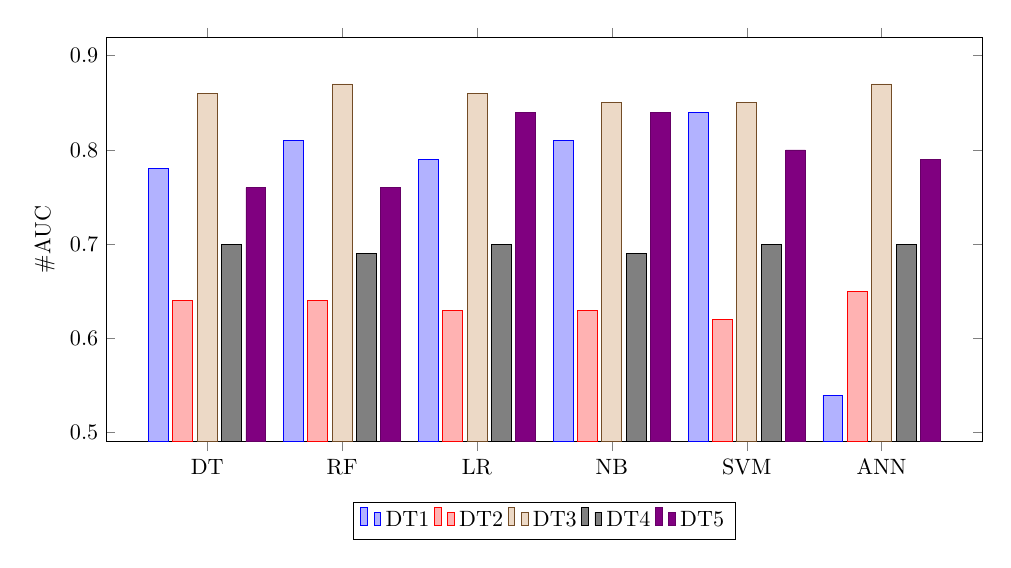
\begin{tikzpicture}[scale=0.8]
 \centering
\begin{axis}[
    height=8cm, width=15.5cm,
    bar width=0.4cm,
    ybar,
    %ybar=5pt,% configures `bar shift'
    bar width=9pt,
    enlargelimits=0.15,
    legend style={at={(0.5,-0.15)},
    anchor=north,legend columns=-1},
    ylabel={\#AUC},
    symbolic x coords={{DT,RF,LR,NB,SVM,ANN}},
    xtick=data,
    %nodes near coords,
    nodes near coords align={vertical},
    ]
\addplot coordinates {(DT,0.78) (RF, 0.81) (LR,0.79)(NB, 0.81)(SVM,0.84)(ANN, 0.54)};
\addplot coordinates{(DT,0.64) (RF, 0.64) (LR,0.63)(NB, 0.63)(SVM,0.62)(ANN, 0.65)};
\addplot coordinates {(DT,0.86) (RF, 0.87) (LR,0.86)(NB, 0.85)(SVM,0.85)(ANN, 0.87)};
\addplot coordinates {(DT,0.70) (RF, 0.69) (LR,0.70)(NB, 0.69)(SVM,0.70)(ANN, 0.70)};
\addplot coordinates {(DT,0.76) (RF, 0.76) (LR,0.84)(NB, 0.84)(SVM,0.80)(ANN, 0.79)};
\legend{DT1,DT2,DT3,DT4,DT5}
\end{axis}
\end{tikzpicture}
\caption{Comparison of the ROC Curves of the classifiers on differents datasets}
\end{figure}
However, on these same datasets, the algorithms often present very low specificities, for example 0.05 on DT1. This shows that our best performing classifiers are only able to predict a single class: either the patient has malaria or he does not, but not in both spots. This is because the DT1 and DT3 datasets are very unbalanced. In fact in these datasets either the number of patients with malaria is greater than those who are not or the opposite is true. Furthermore, we note that on the DT2 and DT4 datasets all the algorithms present specificities and Sensivity that are significant and quite similar. Contrary to what is quoted a little above, on these datasets the algorithms are efficient on the prediction tasks of the two classes. Looking closely at the results in terms of precision, recall and F-measure we observe that the classifiers RF, LR, SVM and ANN generally outperform the others for each dataset. Indeed, for the dataset DT1, which contains observations on patients living in different regions of Senegal, these four classifiers have an accuracy of 99\%, a recall greater than 92\% and an F-measure greater than 95\%. We note the same trend with the DT2 dataset which contains observations on patients living in the same area in Senegal. It can also be noted that RF, LR, SVM and ANN have better precision than the rapid diagnostic test carried out and systematically used in the majority of health structures in Senegal. This observation remains true with DT4 which is a perfectly balanced dataset. In conclusion, it is very difficult or even impossible for us to say definitively which algorithm is more efficient for the task of predicting malaria, but the choice of this one will strongly depend on the choice of the data set. However, this study shows that our classification problem has been taken care of. A method integrating several models and various datasets is necessary

\begin{figure}[!h]
\subfigure[Precision values of compared classifiers on different datasets]{
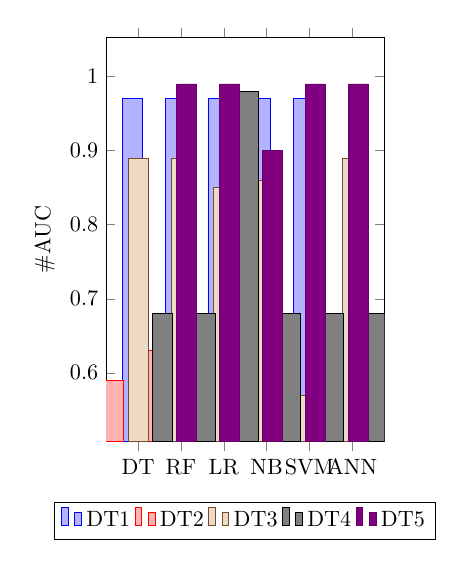
\begin{tikzpicture}[scale=0.8]
 %\centering
\begin{axis}[
    height=8cm, width=6cm,
    bar width=0.4cm,
    ybar,
    %ybar=5pt,% configures `bar shift'
    bar width=9pt,
    enlargelimits=0.15,
    legend style={at={(0.5,-0.15)},
    anchor=north,legend columns=-1},
    ylabel={\#AUC},
    symbolic x coords={{DT,RF,LR,NB,SVM,ANN}},
    xtick=data,
    %nodes near coords,
    nodes near coords align={vertical},
    ]
\addplot coordinates {(DT,0.97) (RF, 0.97) (LR,0.97)(NB, 0.97)(SVM,0.97)(ANN, 0.97)};
\addplot coordinates{(DT,0.59) (RF, 0.63) (LR,0.58)(NB, 0.60)(SVM,0.58)(ANN, 0.59)};
\addplot coordinates {(DT,0.89) (RF, 0.89) (LR,0.85)(NB, 0.86)(SVM,0.57)(ANN, 0.89)};
\addplot coordinates {(DT,0.68) (RF, 0.68) (LR,0.98)(NB, 0.68)(SVM,0.68)(ANN, 0.68)};
\addplot coordinates {(DT,0.99) (RF, 0.99) (LR,0.90)(NB, 0.99)(SVM,0.99)(ANN, 0.99)};
\legend{DT1,DT2,DT3,DT4,DT5}
\end{axis}
\end{tikzpicture}
%\caption{Precision values of compared classifiers on different datasets}
}
\subfigure[Precison, F1-score, specificity values of the classifiers on DT1]{
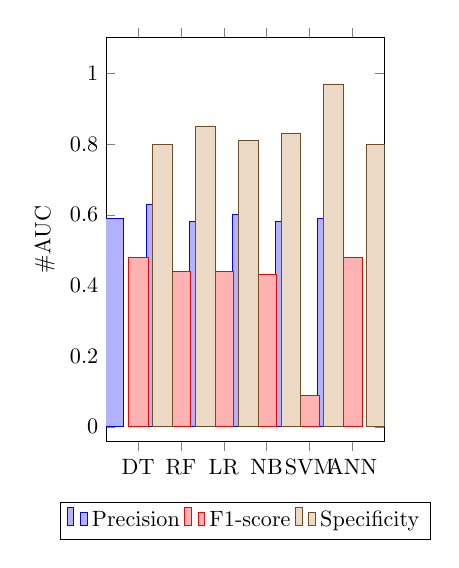
\begin{tikzpicture}[scale=0.8]
\begin{axis}[
    height=8cm, width=6cm,
    bar width=0.4cm,
    ybar,
    %ybar=5pt,% configures `bar shift'
    bar width=9pt,
    enlargelimits=0.15,
    legend style={at={(0.5,-0.15)},
    anchor=north,legend columns=-1},
    ylabel={\#AUC},
    symbolic x coords={{DT,RF,LR,NB,SVM,ANN}},
    xtick=data,
    %nodes near coords,
    nodes near coords align={vertical},
    ]
\addplot coordinates {(DT,0.59) (RF, 0.63) (LR,0.58)(NB, 0.60)(SVM,0.58)(ANN, 0.59)};
\addplot coordinates{(DT,0.48) (RF, 0.44) (LR,0.44)(NB, 0.43)(SVM,0.09)(ANN, 0.48)};
\addplot coordinates {(DT,0.80) (RF, 0.85) (LR,0.81)(NB, 0.83)(SVM,0.97)(ANN, 0.80)};
%\addplot coordinates {(DT,0.68) (RF, 0.68) (LR,0.98)(NB, 0.68)(SVM,0.68)(ANN, 0.68)};
%\addplot coordinates {(DT,0.99) (RF, 0.99) (LR,0.90)(NB, 0.99)(SVM,0.99)(ANN, 0.99)};
\legend{Precision,F1-score,Specificity,DT4}
\end{axis}
%\caption{Precison, F1-score, specificity values of the classifiers on DT1}

\end{tikzpicture}
}
\end{figure}


%\begin{figure}
%\begin{tikzpicture}[scale=0.8]
% \centering
%\begin{axis}[
%    height=8cm, width=15.5cm,
%    bar width=0.4cm,
%    ybar,
%    %ybar=5pt,% configures `bar shift'
%    bar width=9pt,
%    enlargelimits=0.15,
%    legend style={at={(0.5,-0.15)},
%    anchor=north,legend columns=-1},
%    ylabel={\#AUC},
%    symbolic x coords={{DT,RF,LR,NB,SVM,ANN}},
%    xtick=data,
%    %nodes near coords,
%    nodes near coords align={vertical},
%    ]
%\addplot coordinates {(DT,0.59) (RF, 0.63) (LR,0.58)(NB, 0.60)(SVM,0.58)(ANN, 0.59)};
%\addplot coordinates{(DT,0.48) (RF, 0.44) (LR,0.44)(NB, 0.43)(SVM,0.09)(ANN, 0.48)};
%\addplot coordinates {(DT,0.80) (RF, 0.85) (LR,0.81)(NB, 0.83)(SVM,0.97)(ANN, 0.80)};
%%\addplot coordinates {(DT,0.68) (RF, 0.68) (LR,0.98)(NB, 0.68)(SVM,0.68)(ANN, 0.68)};
%%\addplot coordinates {(DT,0.99) (RF, 0.99) (LR,0.90)(NB, 0.99)(SVM,0.99)(ANN, 0.99)};
%\legend{Precision,F1-score,Specificity,DT4}
%\end{axis}
%\end{tikzpicture}
%\caption{Precison, F1-score, specificity values of the classifiers on DT1}
%
%\end{figure}
\section{Conclusion}
In this study, six classifiers using a wide variety of operating procedures have been extensively tested and compared over real world health datasets in order to evaluate their performance for the task of predicting the occurrence or not of Malaria in a patient knowing his signs and symptoms. The results obtained show that the algorithms RF, LR,
SVM with Gaussian kernel and ANN present the best performances in predicting the occurrence or not of Malaria. In addition those four algorithms outperform the Rapid Diagnosis Test which is the standard diagnostic tool largely adopted in the health system in
Senegal. This research has indicated that in practice there is no single best classification tool, but instead the best technique will on the characteristics of the dataset to be analysed. 
Future work consists in the study and the implementation of an ensemble method for predicting the occurrence or not of malaria based on the classifiers offering the best performances in our present study. But also to compare these performances with the ensemble methods for their validation





\bibliographystyle{vancouver}
\bibliography{../biblio}
\end{document}
